\section{Etat de l'art}
\label{sec:etat_de_lart}

\subsection{Evolution logiciel et refactoring}
Pourtant, nombre d'article parlent en introduction de l'importance du refactoring, ce qui inclue le renommage, dans les projets à succès (TODO) mais on obtient pas de chiffres précis.\\

\subsection{Métriques de procédés et évolution logiciel}
Les métriques de procédés (change metrics) permettent de calculer à quel point une entité de code source à été modifiée au cours d'une période donnée. On les utilises usuellement pour prédire les bugs entre deux révisions d'un logiciel, souvent la dernière période. L'objectif étant de prédire les bugs qui apparaitront lors de la prochaine release, elles ne considère que les entités étant toujours présentes à la fin de la période. Elles vont donc se concentrer sur les entités actives lors de la période et que l'on retrouvera à la fin.\\
Un gestionnaire de versions offre plusieurs moyens de calculer ces métriques car il stocke les informations sur les entités modifiés à chaque nouvelle version, l'auteur de ces modifications, la date etc. De plus il permet la récupération du contenu de chaque entité et de l'ensemble d'un projet à une version donnée. Pour calculer ces métriques, il est donc possible d'analyser chaque entités modifiés lors d'une période puis de ne garder uniquement les entités toujours présente à la dernière version de notre période.\\
Nous avons choisi de nous concentrer sur les trois métriques de procédés les plus connues identifiés par Radjenovic et al (TODO) pour mesurer l'impact du renomage: Le nombre de développeurs (NoD), le nombre de modifications (NoC), et le Code Churn (CC).\\
En exemple nous allons considerer $A$, l'ensemble des entités existantes entre deux versions.  TODO
NOD:\\
NOC:\\
CC:\\ 

\begin{figure}[t]
	\centering
	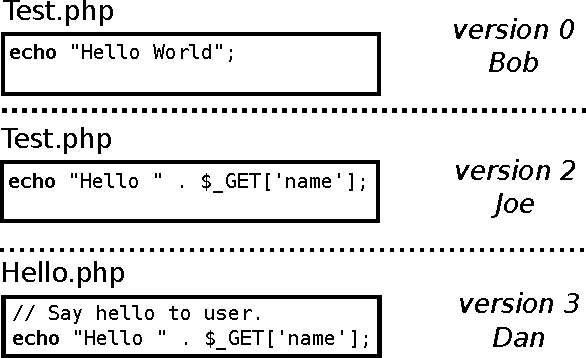
\includegraphics[width=0.8\linewidth,keepaspectratio]{data/figures/example.pdf}
	\caption{Example of a project history. The project is composed of only one file \texttt{Test.php} which is renamed to \texttt{Hello.php} in the last version.}
	\label{fig:example}
\end{figure}

\subsection{Métriques et Renommage}
Comme on l'a expliqué plus tôt, un gestionnaire de versions est très pratique pour calculer les métriques de procédés. Par ailleurs, il faut noter qu'un gestionnaire de version identifie une entité par son chemin + nom de fichier. On en déduit qu'un renommage de cette identité, dans le chemin ou le nom de fichier, aura un impact sur le calcul des métriques. Pour expliquer cet impact, on présente un exemple d'historique d'un logiciel figure 1. Ce projet ne contient qu'une entité, Test.php, qui est renommé en Hello.php dans la dernière version. Dans cet exemple nous calculons NoD, NoC, CC entre la version 1 et 3.\\
La dernière version ne contient qu'une entité. C'est donc cette entité uniquement qui sera considérée. De plus l'identité exacte de cette entité n'aparait que lors de la version 3. Le calcul des métriques est donc trivial, NoD = 1, NoC = 1, CC = 2.\\
Par ailleurs, si on prend en compte le fait que ce fichié a été renommé, il y a trois versions à regarder en ce qui concerne l'entité. etc...TODO\\

\subsection{Métriques et Renommage Existant}
Nous nous somme donc intéressés aux études passées qui pouvaient traiter les métriques de procédés dans la prédiction de bugs, et vérifié si ces études avaient considérés le renommage de fichiers. L'article (TODO) référence 26 articles qui nous intéresse, 15 sur des projets industriels, 11 sur des logiciels open-source. TODO \\

\subsection{Les outils}
Comme nous l'avons vue, il existe un certains nombre de gestionnaires de versions pour effectuer notre détection de renommage, étant donné que nous avons simplement besoin de versions à comparer. Nous avons néhanmoins étudié les VCS potentiels, afin de voir quel VCS sera le plus apte à gérer les renommages. La table1 résume notre étude. TODO Git propose un algorithme de détection automatique de renommage.\\

\subsection{``Origin Analysis''}
L'algorithme utilisé par Git est connu sous sous le nom de ``Origin Analysis'' et est expliqué par Godfrey et al dans les articles, (TODO) (An integrated approach for studying architectural evolution, Tracking Structural Evolution Using Origin Analysis, Using origin analysis to detect merging and splitting of source code entities)
Origin Analysis TODO\\

\begin{table}
\centering
\begin{tabular}{rccc}
\toprule
 & \multicolumn{3}{c}{Renaming handling}\\
\cmidrule{2-4}
& & \multicolumn{2}{c}{Automatic}\\
\cmidrule{3-4}
Tool & Manual & Standard & Optional\\
\midrule
CVS & & &\\
Subversion & $\times$ & &\\
Mercurial & $\times$ & & $\times$\\
Git & & & $\times$\\
\bottomrule
\end{tabular}
\caption{Handling of renaming of the main VCS tools.}
\label{tab:vcs}
\end{table}
